\section{Electrons in a Periodic Potential - Tight Binding Approximation}
\subsection{Review and Examples of Band Structure}
We recall that a weak perturbation has no effect on the electron spectrum except at the degeneracy points. At these points, the perturbation results in a gap at these degeneracy points of magnitude $2\abs{U_G}$. 

We did this for one specific degeneracy point (Bragg plane), but there will be many such points. The free electron parabola gets proken up into many such disjoint pieces. We can picture this in the extended zone scheme (pictures $-\infty < k < \infty$), or the reduced zone scheme (pictures the first Bruilloin zone with many levels), or the repeated zone scheme (copying over the structure in the first Bruilloin zone multiple times throughout space) as pictured below.

\begin{figure}[htbp]
    \centering
    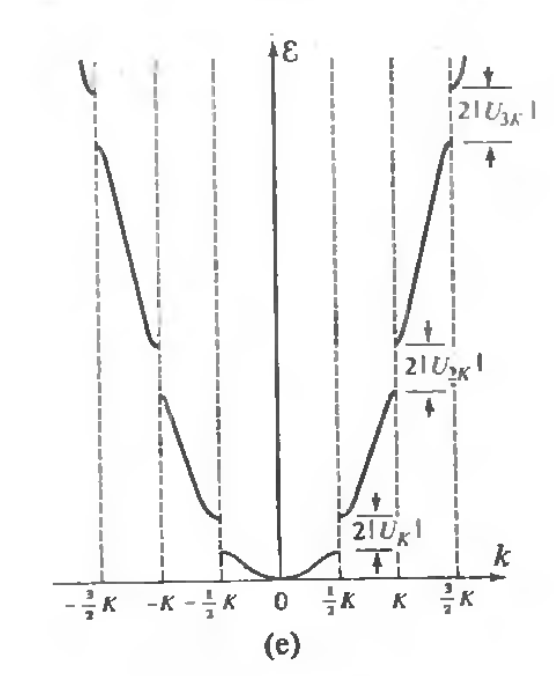
\includegraphics[scale=0.5]{Images/fig-extendedzonescheme.png}
    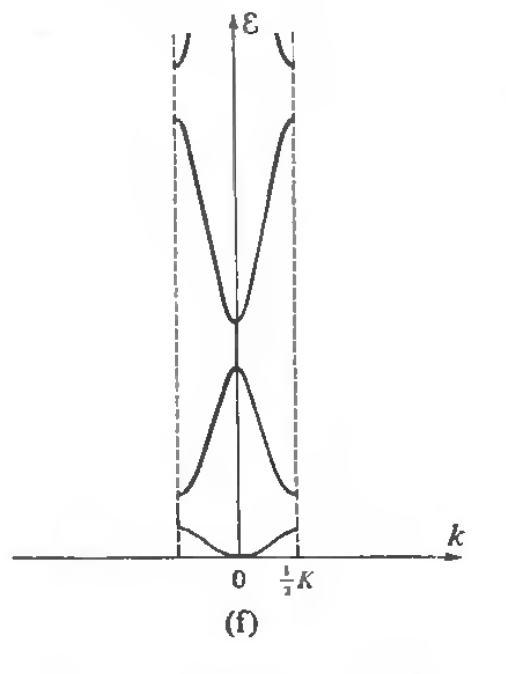
\includegraphics[scale=0.5]{Images/fig-reducedzonescheme.png}
    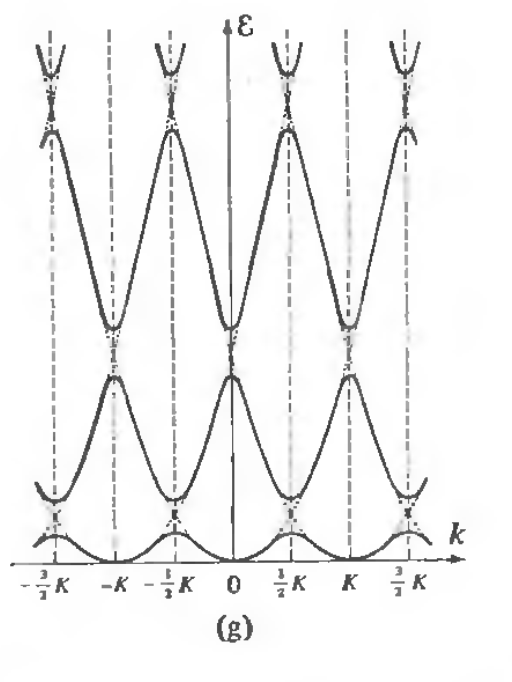
\includegraphics[scale=0.5]{Images/fig-repeatedzonescheme.png}
    \caption{Sketch of the extended (left), reduced (center), and repeated (right) zone schemes for describing the electron dispersion under a weak periodic perturbation. Figures reproduced without permission from Ashcroft and Mermin.}
    \label{fig-extendedreducedrepeatedzoneschemes}
\end{figure}

In three dimensions, the analysis proceeds in the same way (but there are more levels at the same $\v{k}$). If the Fermi energy lies inside of the band, we have a metal (e.g. aluminum), and if we have a Fermi energy inside of the gap, we have an insulator (e.g. silicon).

An important 2D example is graphene; we consider carbon atoms in a honeycomb lattice, which can be viewed as a triangular Bravais lattice with a two point basis. It has a hexagonal Bruillon zone, and the band structure looks fairly free electron. Near the $K$ point (corner of the Bruillon zone), there is a protection (from time reversal and inversion symmetry) and there is the realization of dirac dispersion near the $K$ points; here we see behavior like massless particles, with zero curvature. Electrons near these $K$ points are in some sense massless. This is a kind of band structure that we could \emph{not} get from the weak periodic potential approximation, as the periodic potential is not weak. It also motivates our next topic, which is the tight-binding approximation (which is successful for (e.g.) graphene).

\subsection{Tight-Binding Approximation}
We consider again a periodic potential, this time the case where we have a periodic Coloumb potential. If we focus on the highly excited wavefunctions at each site, we have an exponentially decaying wavefunction centered at each well. If only the exponentially small tails of the wavefunctions overlap, then we can think of the system as electrons sitting in their orbitals, and being subject to a small perturbation that allows them to tunnel from one well to another. In some sense it is the complete opposite of the weak potential approximation. There we started with free electrons and treated the potential as a perturbation. Here, we assume electrons are tightly bound in atomic orbitals; tunnelling (a.k.a. ``hopping'') occurs due to small wavefunction overlap (the perturbation). 

\begin{figure}[htbp]
    \centering
    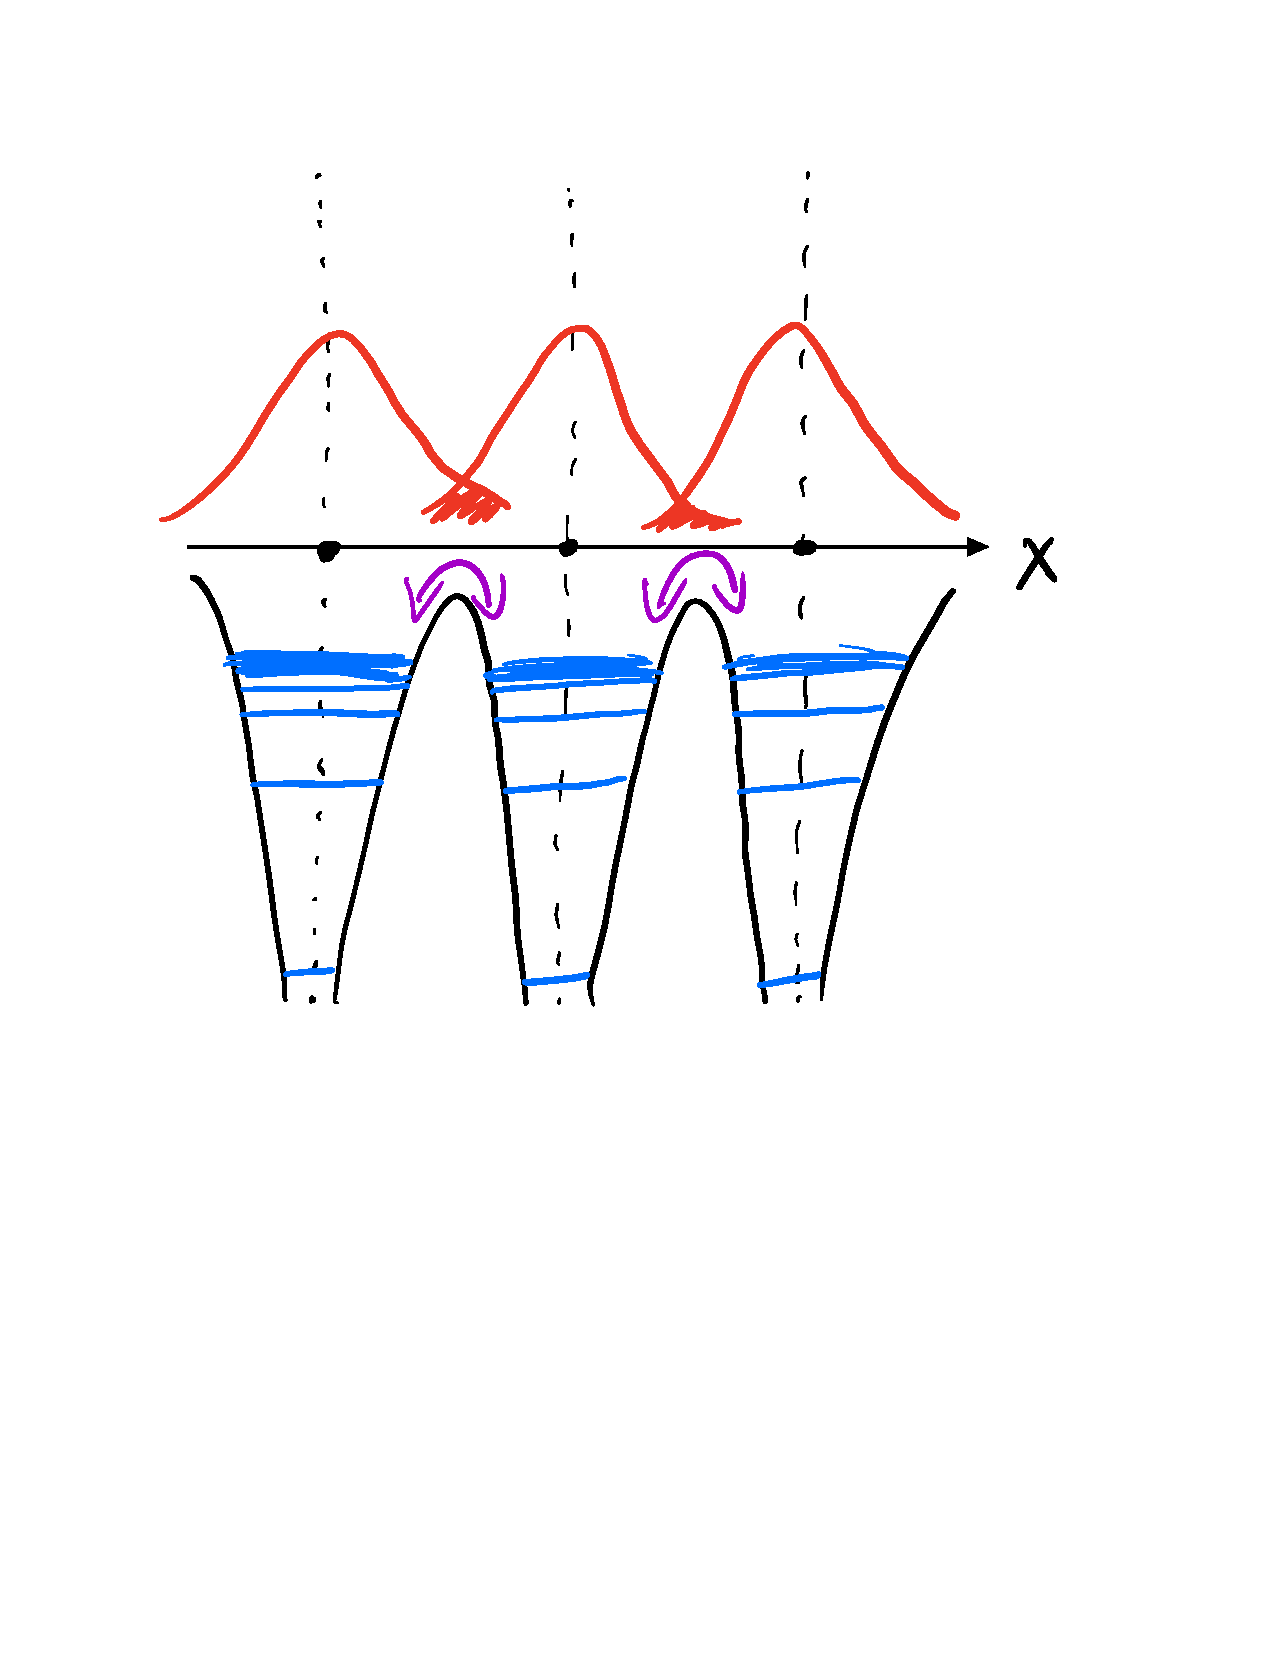
\includegraphics[scale=0.5]{Images/fig-tightbindingcartoon.pdf}

    \caption{Cartoon sketch of the tight-binding approximation. We have per-site wavefunctions (arising from a Coloumb potential, or some other strong per-site potential) that are centered at each site of the lattice that ``strongly bind'' the electrons. There is overlap between the per-site wavefunctions that leads to hopping in between the sites.}
    \label{fig-tightbindingcartoon}
\end{figure}

We have the Hamiltonian:
\begin{equation}
    H = -\frac{\hbar^2\nabla^2}{2m} + \sum_i U_{at}(\v{r} - \v{R}_i)
\end{equation}
We work in the basis of atomic wavefunctions $\phi_n(\v{r})$, which satisfy:
\begin{equation}
    H_{at}\phi_n = E_n\phi_n, \quad H_{at} = -\frac{\hbar^2\nabla^2}{2m} + U_{at}(\v{r})
\end{equation}
we assume that the $\phi_n$s are known. This is our starting point. We write the full Hamiltonian in second quantization notation using the $\phi_n$ basis. We introduce operators $c_n^\dag (\v{R}_i)$ which creates an electron in state $\phi_n(\v{r} - \v{R}_i)$ represented as $\ket{n, \v{R}_i}$. Then, the most general tight binding Hamiltonian can be written as:
\begin{equation}
    \hat{H} = \sum_{m, n}\sum_{i, j}\bra{n, \v{R}_i}H\ket{m, \v{R}_j}c^\dag_n(\v{R}_i)c_m(\v{R}_j)
\end{equation}
$c^\dag_n(\v{R}_i)c_m(\v{R}_j)$ precisely destroys one electron at energy $E_m$ at position $\v{R}_j$ and creates one at energy $E_n$ at position $\v{R}_i$. The matrix elements $\bra{n, \v{R}_i}H\ket{m, \v{R}_j} = t_{ij}^{mn}$ give the amplitudes for this process to occur.  

This general form is generally not super useful unless more about the matrix elements are known. Fortunately, because the atomic wavefunctions $\phi_n(\v{r})$ decay as $\sim e^{-r/a_0}$, we expect the overlap between the wavefunctions is only appreciable between a few nearest neighbours, and the rest are negligeble. So, the matrix elements $t_{ij}^{mn}$ are negligeble when $\abs{\v{R}_i - \v{R}_j} \gg a_0$. In practice, it is usually sufficient to include first (potentially second or third) neighbour hopping.

Tight binding models can be solved for any order of these hoppings, but low order ones have very simple solutions. Note that we will not go into the band structure calculations of the $t_{ij}^{mn}$ matrix elements here; but there are many textbooks and packages written specifically about this topic. There are well-established techniques, but they require detailed knowledge of atomic orbitals. This is often difficult to do by hand; however, they can often be constrained by symmetries.

\begin{figure}[htbp]
    \centering
    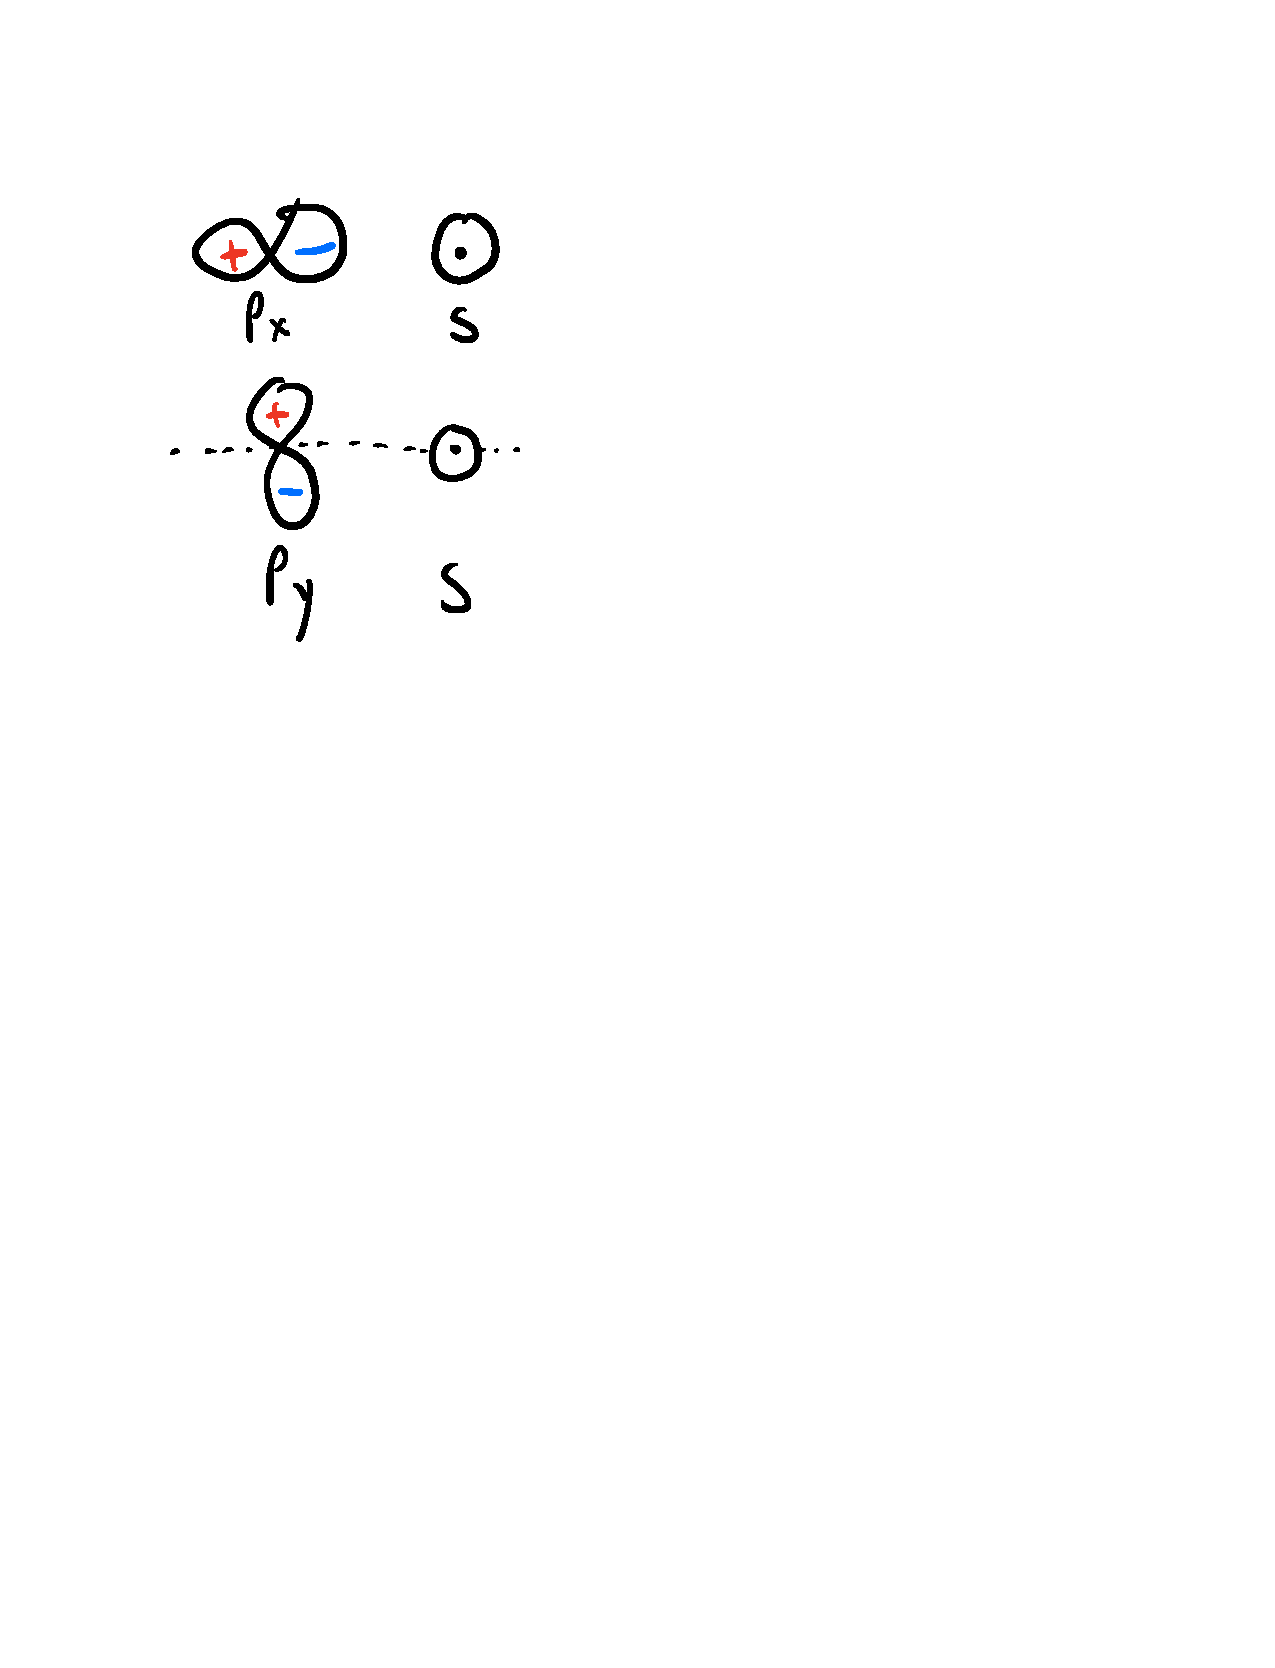
\includegraphics[scale=0.5]{Images/fig-orbitaloverlapsymmetries.pdf}
    
    \caption{The overlap matrix elements $t_{ij}^{mn}$ can often be constrained by symmetries. When looking at the overlap of $p_x$ and $s$, symmetry constraints give us no information. However, when looking at the overlap of $p_y$ and $s$, the overlap integral is odd under the interchange $y \leftrightarrow -y$ and so we conclude that the matrix element vanishes.}
    \label{fig-orbitaloverlapsymmetries}
\end{figure}


\subsection{Example - Single non-degenerate orbital in 2D}
\begin{figure}[htbp]
    \centering
    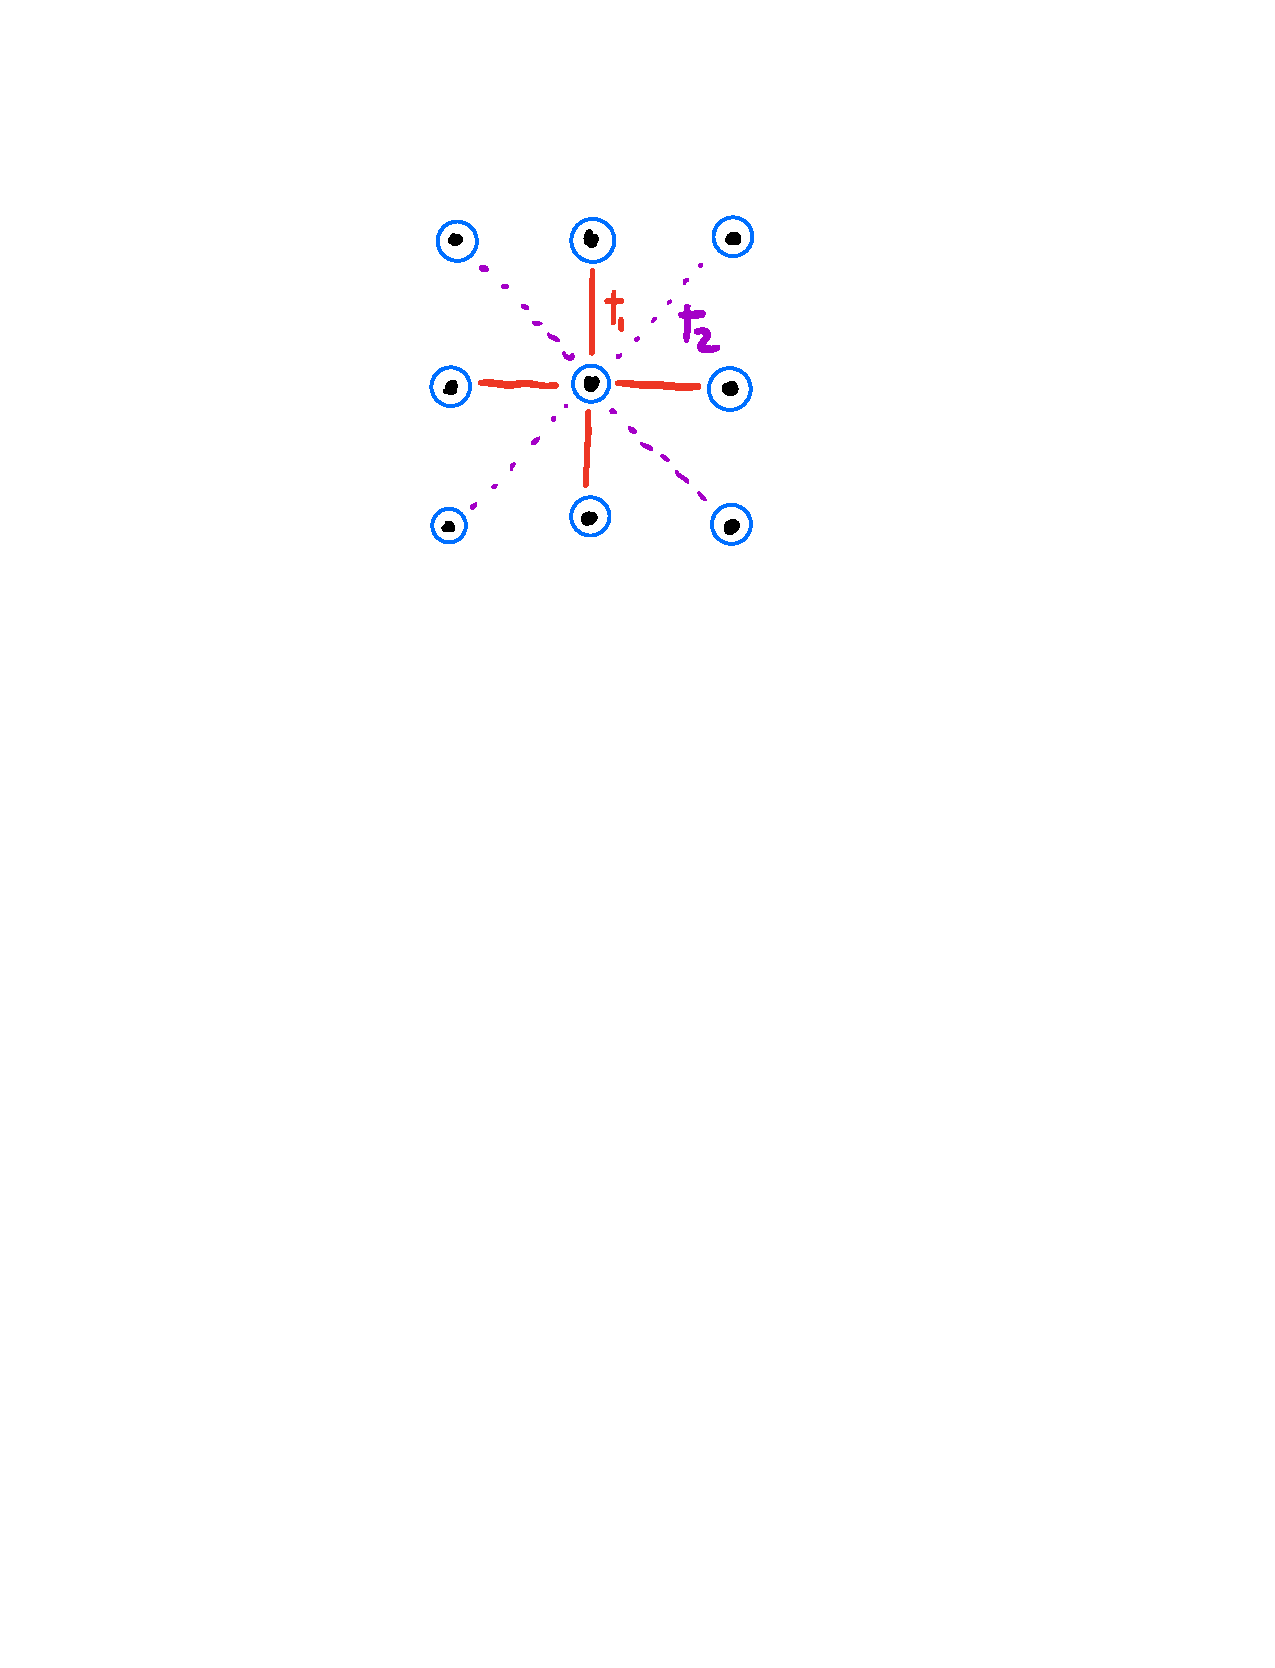
\includegraphics[scale=0.7]{Images/fig-2dtightbindingsquarelattice.pdf}
    
    \caption{Sketch of a 2D square lattice with a single non-degenerate orbital at each site. The interactions to consider will be the nearest neighbour interactions $(t_1)$ and the next-nearest interactions $(t_2)$. The next-next nearest neighbour interactions and further can be neglected.}
    \label{fig-2dtightbindingsquarelattice}
\end{figure}
In this scenario our tight-binding Hamiltonian looks like:
\begin{equation}
    \hat{H} = \sum_i E_i c^\dag(\v{R}_i)c(\v{R}_i) - \sum_{i \neq j}t_{ij}c^\dag(\v{R}_i)c(\v{R}_j)
\end{equation}
here, $E_i$ is the ``on-site'' energy. We will take $E_i = \e_0$ for all $i$ in our monoatomic lattice. for $t_{ij}$ we consider only first and second neighbours as indicated in the figure:
\begin{align*}
    t_{ij} = \begin{cases}
        t_1 & \text{first neighbour}
        \\ t_2 & \text{second neighbour}
        \\ 0 & \text{otherwise}
    \end{cases}
\end{align*}
With this we can rewrite:
\begin{equation}
    \hat{H} = \e_0 \sum_i \e_0 c^\dag(\v{R}_i)c(\v{R}_i) - \sum_{i, \gv{\delta}}t_{\gv{\delta}}c^\dag(\v{R}_i + \gv{\delta})v(\v{R}_i)
\end{equation}
this is often a useful rewrite as in many cases the hopping terms do not depend on both lattice positions $i, j$ but only the difference between them $\gv{\delta}$. $\gv{\delta}$ here are vectors that point from a site to its first and second neighbour. We will see that a Fourier transform immediately solves this type of simple problem:
\begin{equation}
    \begin{split}
        c(\v{R}_i) &= \frac{1}{\sqrt{N}}\sum_\v{k}e^{i\v{k} \cdot \v{R}_i}c_\v{k}
        \\ c^\dag(\v{R}_i) &= \frac{1}{\sqrt{N}}\sum_\v{k}e^{-i\v{k} \cdot \v{R}_i}c^\dag_\v{k}
    \end{split}
\end{equation}
our Fourier transformed Hamiltonian takes the form:
\begin{equation}
    \begin{split}
        \hat{H} &= \e_0\sum_{\v{k}, \v{k}'}c^\dag_\v{k}c_{\v{k}'}\frac{1}{N}\sum_{\v{R}_i}e^{-i\v{R}_i\cdot(\v{k} - \v{k}')} - \sum_{\v{k}, \v{k}'}c^\dag_\v{k}c_{\v{k}'}\frac{1}{N}\sum_{i, \gv{\delta}}t_{\gv{\delta}}e^{-i\v{R}_i\cdot(\v{k} - \v{k}') - i\gv{\delta}\cdot \v{k}}
        \\ &= \e_0\sum_{\v{k}}c^\dag_\v{k}c_{\v{k}} - \sum_{\v{k}}c^\dag_\v{k}c_{\v{k}}\left(\sum_{\gv{\delta}}t_{\gv{\delta}}e^{- i\gv{\delta}\cdot \v{k}}\right)
    \end{split}
\end{equation}
and so:
\begin{equation}
    \hat{H} = \sum_{\v{k}}\e(\v{k})c^\dag_{\v{k}}c_\v{k}, \quad \e(\v{k}) = \e_0 - \sum_{\gv{\delta}}t_{\gv{\delta}}e^{-i\v{k} \cdot \gv{\delta}}
\end{equation}
Actually the solution we write above works for any tight binding model. We can evaluate the energies for our case specifically using that $\gv{\delta}_1 = a(\pm \xhat, \pm \yhat)$ and $\gv{\delta}_2 = a(\xhat \pm \yhat, -\xhat \pm \yhat)$. This yields:
\begin{equation}
    \e(\v{k}) = \e_0 - 2t_1(\cos(ak_x) + \cos(ak_y)) - 2t_2(\cos(a(k_x + k_y)) + \cos(a(k_x - k_y)))
\end{equation}

For simplicity, let us illustrate the case with $t_2 = 0$. We sketch the lines of constant energy for the dispersion:
\begin{align*}
    \e(\v{k}) = \e_0 - 2t_1(\cos(ak_x) + \cos(ak_y))
\end{align*}

\begin{figure}[htbp]
    \centering
    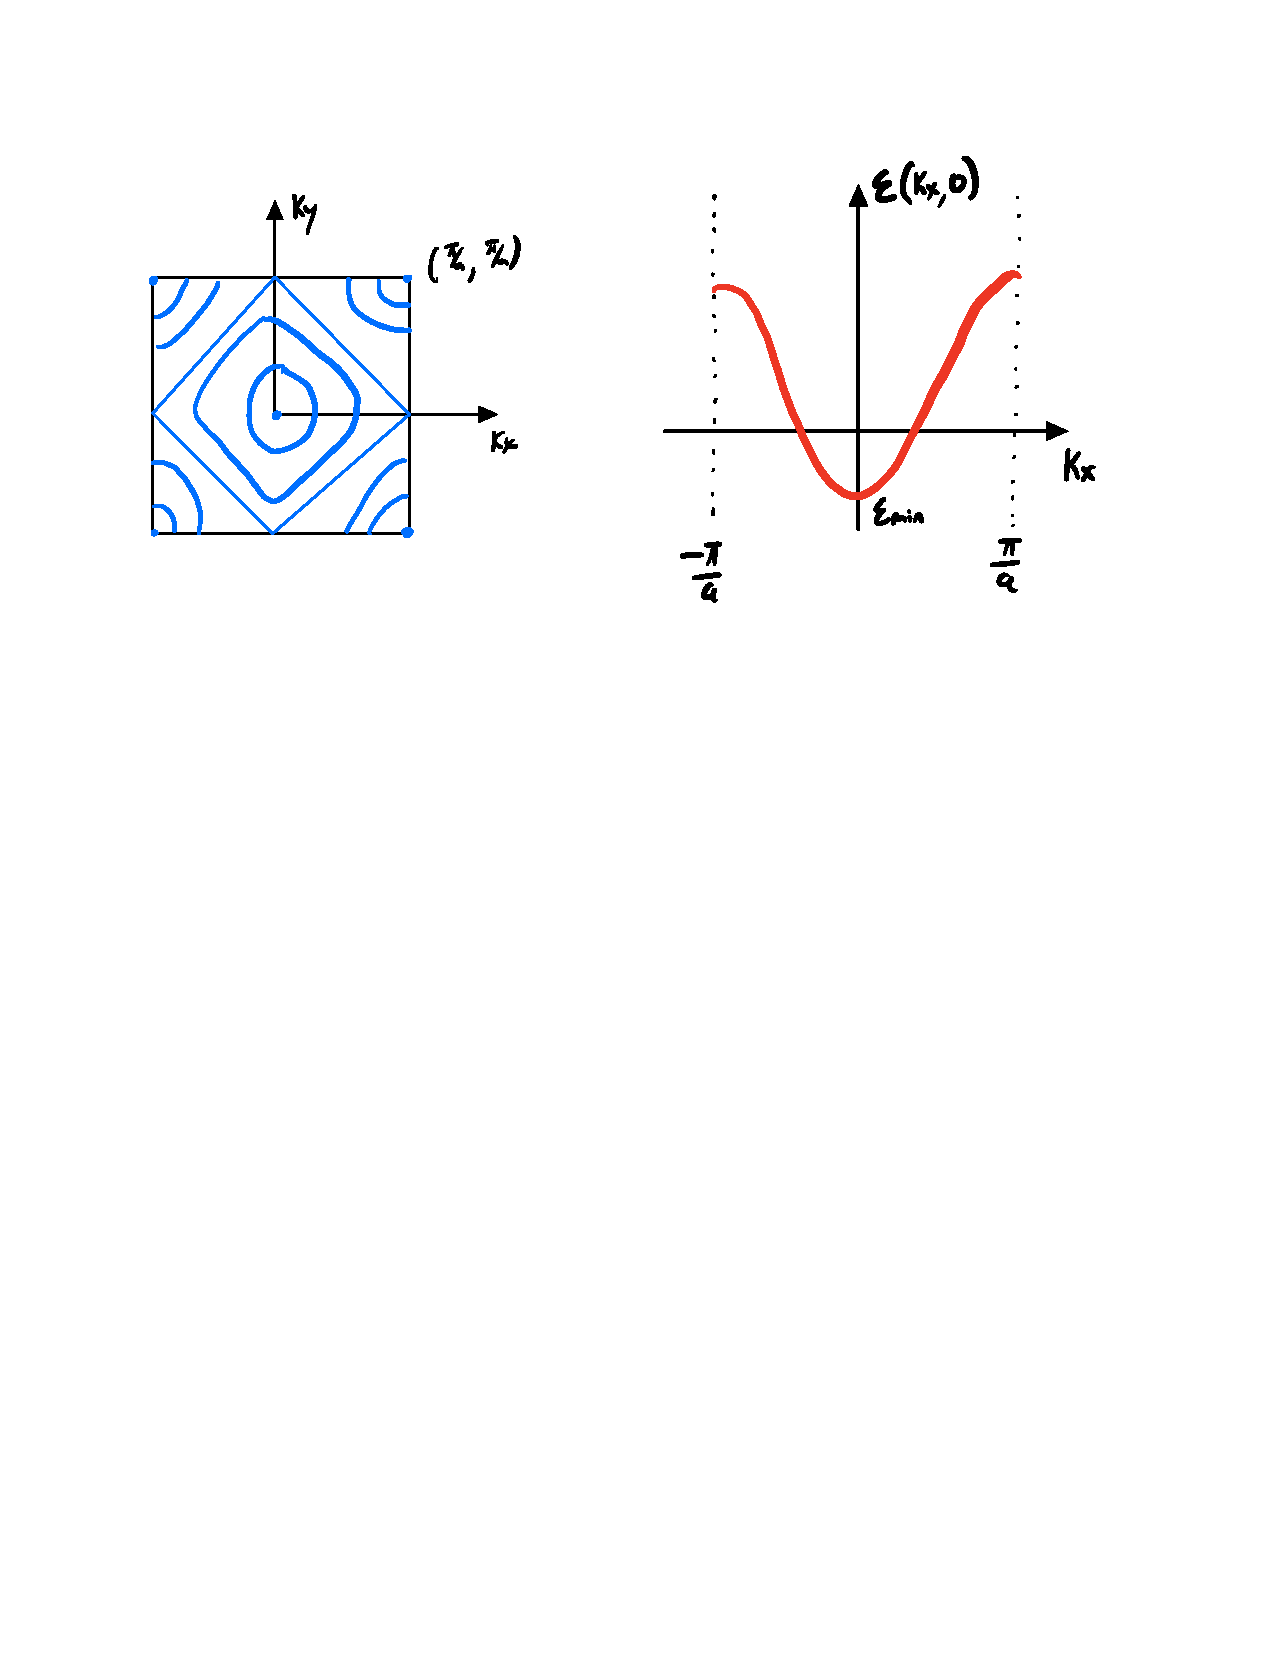
\includegraphics[scale=0.7]{Images/fig-2dtightbindingsquarelatticedispersion.pdf}
    
    \caption{Lines of constant energy for the 2D tight-binding square lattice with one non-degenerate orbital (left) and plot of energy vs. $k_x$ for fixed $k_y = 0$ (right).}
    \label{fig-2dtightbindingsquarelatticedispersion}
\end{figure}

We find that $\e_{\text{min}} = \e(\v{k} = \v{0}) = \e_0 - 4t$ and $\e_{\text{max}} = \e(\v{k} = (\frac{\pi}{a}, \frac{\pi}{a})) = \e_0 + 4t$. The bandwidth is $W = \e_{\text{max}} - \e_{\text{min}} = 8t$. 

A standard undergraduate question: if we have a 2D square lattice and each atom contributes one electron, do we have a metal or an insulator? To answer this, we recall that the number of $k$ states in the band is equal to the number of unit cells in the crystal.

On the face of it, it seems like all of the $N$ states would be filled with electrons so we would have an insulator. But taking into account spin, there are $2N$ states, so we only fill half of the states, corresponding to all of the states inside of the diamond. This meets the definition of a metal!

\begin{figure}[htbp]
    \centering
    
    \caption{<caption>}
    \label{<label>}
\end{figure}

\subsubsection{Effective Mass}
The effective mass for these electrons can be defined near either the minima or the maxima of the dispersion by expanding it to second order in momenta and study the long wavelength behavior.
\begin{enumerate}[(i)]
    \item Near $\v{k} = \v{0}$, we can expand:
    \begin{equation}
        \e(\v{k}) = \e_0 - 2t_1(1 - \frac{(ak_x)^2}{2} + \ldots + 1 - \frac{(ak_y)^2}{2} + \ldots) = (\e_0 - 4t_1) + t_1a^2k^2 + \ldots 
    \end{equation}
    In the literature, often $t_1a^2k^2$ is written as $\frac{\hbar^2 k^2}{2m^*}$ with $m^* = \frac{\hbar^2}{2t_1a^2}$ the effective mass. In principle this could be larger or smaller than the real electron mass, and in the literature when things such as ``heavy electrons'' are discussed, these are compounds where the band mass of the electrons is heavy. In conclusion, near $\v{k} = 0$ (the $\Gamma$ point) the tight-binding electron behaves as a particle of mass $m^*$.

    \item Near $\v{k} = \left(\frac{\pi}{a}, \frac{\pi}{a}\right) \equiv \v{K}$, we expand:
    \begin{equation}
        \e(\v{k} + \v{K}) = (e_0 + 4t_1) - t_1a^2k^2 + \ldots
    \end{equation}
    where we now have the effective mass $m^* = -\frac{\hbar^2}{2t_1 a^2}$. The effective mass is negative! The carriers are holes.
\end{enumerate}

\subsubsection{Band Velocity}
The group velocity is given by:
\begin{equation}
    \v{v}_\v{k} = \frac{1}{\hbar}\dpd{\e(\v{k})}{\v{k}} = \frac{2t_1a}{\hbar}(\sin(ak_x), \sin(ak_y))
\end{equation}

\begin{figure}[htbp]
    \centering
    
    \caption{<caption>}
    \label{<label>}
\end{figure}

Near $\v{k} = 0$, we have $\v{v}_\v{k} \approx \frac{2t_1a^2}{\hbar}\v{k}$. This is as expected for a free particle of mass $m^*$. Near $k_x = \frac{\pi}{a}$, we have $\v{v}_\v{k} = -\frac{2ta^2}{\hbar}\delta k_x$. This is very odd. The velocity is opposite to the change in momentum. This is however consistent with the effective mass being negative.

One may ask what makes electrons behave in this strange way. The intuition of free space is violated here as the electron is not moving in free space (it is in the tight-binding model)! In the long wavelength limit the free space analogy may hold, but in other parts of the Bruillon zone this is simply not the case.

Another point - this shows why it is important to distinguish between momentum and crystal momentum. Here we have crystal momentum, and we can see it really does not behave as we conventionally understand momentum.

\subsection{Example - Lattice with a Basis (Dimerized chain)}
\begin{figure}[htbp]
    \centering
    
    \caption{<caption>}
    \label{<label>}
\end{figure}

Our unit cell now contains two atoms, and is of length $2a$. Every atom in the chain can be labelled by the position of the unit cell and with $1/2$. We therefore write the Hamiltonian in second quantization notation as:
\begin{equation}
    H = \e_0 \sum_i \left[c_1^\dag(R_i)c_1(R_i) + c_2^\dag(R_i)c_2(R_i)\right] + t\sum_i\left[c_1^\dag(R_i)c_2(R_i + a) + h.c.\right] + t'\sum_i \left[c_1^\dag(R_i)c_2(R_i - a) + h.c.\right]
\end{equation}
where $c_1^\dag c_2$ describes a hop from site 2 to site 1 and h.c. the opposite. We solve this via a Fourier transform:
\begin{align*}
    c_\alpha(r) = \frac{1}{\sqrt{N}}\sum e^{ikr}c_{\alpha k}
\end{align*}
$\alpha = 1, 2$:
\begin{equation}
    H = \e_0\sum_{\alpha, k}c^\dag_{k, \alpha}c_{k, \alpha} + t\sum_k \left(c^\dag_{1k}c_{2k}e^{ika} + h.c.\right) + t'\sum_k \left(c^\dag_{1k}c_{2k}e^{-ika} + h.c.\right)
\end{equation}
Two solve, define a two-component spinor:
\begin{align*}
    \chi_k = \m{c_{1k} \\ c_{2k}}, \quad \chi_k^\dag = \m{c^\dag_{1k} & c^\dag_{2k}}
\end{align*}
and express the Hamiltonian (setting $a = 1$):
\begin{equation}
    H = \sum_k \chi_k^\dag h_k\chi_k, \quad  h_k = \m{\e_0 & te^{ik} + t'e^{-ik} \\ te^{-ik} + t'e^{ik} & \e_0}
\end{equation}
We diagonalize this matrix, setting $\det(j_k - \e\II) = 0$. We get a secular equation:
\begin{align*}
    (\e_0 - \e)^2 - (te^{ik} + t'e^{-ik})(te^{-ik} + t'e^{ik}) = 0
\end{align*}
When we solve the quadratic equation for $\e$, we find:
\begin{equation}
    \e = \e_0 \pm \sqrt{t^2 + t'^2 + 2tt'\cos(2k)}
\end{equation}
so the band structure will be composed of two bands.

Now, suppose that each atom in this dimerized chain donates exactly one electron. Do we have a metal or insulator? Each unit cell has two atoms. So, if each atom contributes one electron, the bottom band is completely filled (with $N$ electrons) and the top band is completely unfilled. So we have an insulator.

Another question - what happens if the atoms we make them now identical? The gap closes - but this is something for the reader to think about. This ends the discussion of the tight binding model, and we do other things starting monday.